\section*{(17\textordfeminine\ aula) --- Partícula sob Força Constante}

\subsection*{Partícula sob Força Constante}

Um outro potencial que permite solução exata em 1D é $V(x) = -Fx$, o potencial de uma força constante.

Em Mecânica Clássica discutimos esse potencial quando estudamos o problema da queda livre, por exemplo.

\subsection*{Mecânica Clássica}

\begin{equation}
    H(x,p) = \frac{p^2}{2m} - Fx \qquad (F \text{ constante})
\label{eq:aula17_H_classica}
\end{equation}

\begin{equation}
    \dot{x} = \frac{p}{m} \qquad \text{e} \qquad \dot{p} = F
\label{eq:aula17_eqs_hamilton}
\end{equation}
são as equações de Hamilton.

Eliminando $p(t)$ encontramos a equação de Newton
\begin{equation}
    \ddot{x} = \frac{F}{m} \quad \Longrightarrow \quad
    \begin{cases}
        x(t) = x(0) + \dot{x}(0)\, t + \dfrac{1}{2}\dfrac{F}{m} t^2 \\[2mm]
        p(t) = m\dot{x} = \underbrace{m\dot{x}(0)}_{p_0} + Ft
    \end{cases}
\label{eq:aula17_eq_newton}
\end{equation}

Trata-se do movimento uniformemente acelerado. A energia total é conservada e pode ter qualquer valor em $(-\infty, \infty)$.
\begin{equation}
    E = \frac{p_0^2}{2m} - Fx_0
\label{eq:aula17_energia_classica}
\end{equation}

\subsection*{Mecânica Quântica}

Esse potencial é interessante pois a equação de autovalor do operador $\hat{H}$ é mais facilmente resolvida na base $\ket{p}$ do que na base $\ket{x}$.

Da forma do potencial antecipamos um espectro contínuo, com $E \in (-\infty, \infty)$, e com autovalores \textbf{NÃO-DEGENERADOS}.

\begin{center}
\begin{tikzpicture}[scale=1]
    \draw[->] (-3,0) -- (3,0) node[right] {$x$};
    \draw[->] (0,-1.6) -- (0,2.2) node[above] {$V(x)$};
    \draw[thick] (-2.5,1.25) -- (2.5,-1.25) node[right] {};
    \node at (2.7,-1.4) {$-Fx$};
    \draw[thick] (-2.3,1.0) -- (2.3,1.0);
    \node[right] at (2.3,1.0) {$E$ (não degenerado)};
\end{tikzpicture}
\end{center}

\begin{equation}
    \left( \frac{\hat{p}^2}{2m} - F\hat{x} \right) \ket{E} = E \ket{E}
\label{eq:aula17_autovalor_H}
\end{equation}

Tomando o produto interno com $\bra{p}$:
\begin{equation}
    \frac{p^2}{2m}\psi_E(p) - i\hbar F \frac{d\psi_E}{dp} = E\, \psi_E(p)
\label{eq:aula17_edo_p}
\end{equation}

Uma EDO do 1\textsuperscript{o} grau, com solução
\begin{equation}
    \braket{p}{E} = \psi_E(p) = A \exp\left[ \frac{iEp}{F\hbar} - \frac{ip^3}{6mF\hbar} \right]
\label{eq:aula17_psiE_sem_norm}
\end{equation}

O fato de só aparecer 1 constante arbitrária (pois a EDO era de 1\textsuperscript{a} ordem) indica que o autovalor é \textbf{NÃO DEGENERADO}, como sabíamos.

Impomos a normalização $\braket{E}{E'} = \delta(E - E')$:
\begin{align}
    \braket{E}{E'} &= \int_{-\infty}^{\infty} dp\, \braket{E}{p}\braket{p}{E'} \notag \\
    &= \int_{-\infty}^{\infty} dp\, A^2\, e^{i(E'-E)p/F\hbar} = A^2\, 2\pi\, \delta\!\left( \frac{E'-E}{F\hbar} \right) \notag \\
    &= A^2\, 2\pi F\hbar\, \delta(E-E')
\label{eq:aula17_normalizacao}
\end{align}

Escolhemos $A = \sqrt{\dfrac{1}{2\pi\hbar F}}$ para obter a normalização desejada.

\begin{equation}
    \boxed{\psi_E(p) = \frac{1}{\sqrt{2\pi\hbar F}} \exp\left[ \frac{iEp}{F\hbar} - \frac{ip^3}{6mF\hbar} \right]}
\label{eq:aula17_psiE_normalizada}
\end{equation}

\subsection*{Operador de Evolução na Base $\ket{p}$}

Podemos obter o operador de evolução na base $\ket{p}$:
\begin{align}
    \bra{p} e^{-i\hat{H}t/\hbar} \ket{p'} &= \int_{-\infty}^{\infty} dE\, e^{-iEt/\hbar} \braket{p}{E}\braket{E}{p'} \qquad \left( \hat{1} = \int_{-\infty}^{\infty} dE \ket{E}\bra{E} \right) \notag \\
    &= \int_{-\infty}^{\infty} dE\, e^{-iEt/\hbar} \frac{1}{2\pi\hbar F} \exp\left[ \frac{iE(p-p')}{F\hbar} - i\frac{p^3 - p'^3}{6mF\hbar} \right] \notag \\
    &= \frac{2\pi}{2\pi\hbar F}\, \delta\!\left( \frac{p-p'}{F\hbar} - \frac{t}{\hbar} \right) e^{-i\frac{p^3-p'^3}{6mF\hbar}} \notag \\
    &= \delta(p - p' - Ft)\, e^{-i\frac{p^3-p'^3}{6mF\hbar}}
\label{eq:aula17_operador_evolucao_p}
\end{align}

Esse ``propagador'' não é o propagador usual, que é $\bra{x} e^{-i\hat{H}t/\hbar} \ket{x'}$. Ele é usado quando temos $\braket{p}{\Psi(0)} = \Psi(p,0)$, a função de onda inicial no \textbf{ESPAÇO p}.

\begin{equation}
    \ket{\Psi(t)} = e^{-i\hat{H}t/\hbar} \ket{\Psi(0)}
\label{eq:aula17_evolucao_ket}
\end{equation}

\begin{equation}
    \braket{p}{\Psi(t)} = \int_{-\infty}^{\infty} dp'\, \bra{p} e^{-i\hat{H}t/\hbar} \ket{p'} \braket{p'}{\Psi(0)}
\label{eq:aula17_psi_t_p}
\end{equation}

\begin{equation}
    \Psi(p,t) = \int_{-\infty}^{\infty} dp'\, \bra{p} \hat{U}(t) \ket{p'}\, \Psi(p',0)
\label{eq:aula17_psi_t_p_U}
\end{equation}

\subsection*{Exemplo: Pacote Gaussiano Inicial}

Por exemplo, para o pacote inicial
\begin{equation}
    \braket{x}{\Psi(0)} = \Psi(x,0) = \left( \frac{1}{\pi\Delta^2} \right)^{1/4} e^{ip_0 x/\hbar}\, e^{-x^2/2\Delta^2}
\label{eq:aula17_pacote_inicial_x}
\end{equation}

Temos
\begin{align}
    \Psi(p,0) = \braket{p}{\Psi(0)} &= \int_{-\infty}^{\infty} dx\, \braket{p}{x}\braket{x}{\Psi(0)} \notag \\
    &= \int_{-\infty}^{\infty} dx\, \frac{e^{-ipx/\hbar}}{\sqrt{2\pi\hbar}}\, \Psi(x,0) \notag \\
    &= \left( \frac{\Delta^2}{\hbar^2\pi} \right)^{1/4} \exp\left[ -\frac{(p-p_0)^2\Delta^2}{2\hbar^2} \right]
\label{eq:aula17_psi_p0}
\end{align}

Esse pacote inicial evolui com o tempo para
\begin{align}
    \Psi(p,t) &= \int_{-\infty}^{\infty} dp'\, \underbrace{\delta(p-p'-Ft)\, e^{-i\frac{p^3-p'^3}{6mF\hbar}}}_{\bra{p}\hat{U}(t)\ket{p'}}\, \underbrace{\left( \frac{\Delta^2}{\hbar^2\pi} \right)^{1/4} e^{-\frac{(p'-p_0)^2\Delta^2}{2\hbar^2}}}_{\Psi(p',0)} \notag \\
    &= \left( \frac{\Delta^2}{\hbar^2\pi} \right)^{1/4} \exp\left[ -i\frac{p^3 - (p-Ft)^3}{6mF\hbar} - \frac{(p-Ft-p_0)^2\Delta^2}{2\hbar^2} \right]
\label{eq:aula17_psi_p_t}
\end{align}

Vemos que a distribuição de momenta se desloca rigidamente no eixo $p$:
\begin{equation}
    |\Psi(p,t)|^2 = \left( \frac{\Delta^2}{\hbar^2\pi} \right)^{1/2} e^{-(p-Ft-p_0)^2\Delta^2/\hbar^2}
\label{eq:aula17_modulo_psi_p_t}
\end{equation}

\begin{center}
\begin{tikzpicture}[scale=1]
    \draw[->] (-1,0) -- (8,0) node[right] {$p$};
    \draw[domain=-0.3:1.3,smooth,variable=\x] plot ({\x},{1.8*exp(-20*(\x-0.5)^2)});
    \draw[domain=4.7:6.3,smooth,variable=\x] plot ({\x},{1.8*exp(-20*(\x-5.5)^2)});
    \node[below] at (0.5,0) {$p_0$};
    \node[below] at (5.5,0) {$p_0+Ft$};
    \draw[<->] (-0.1,2.1) -- (1.1,2.1);
    \node[above] at (0.5,2.1) {$\hbar/\Delta$};
    \draw[<->] (4.9,2.1) -- (6.1,2.1);
    \node[above] at (5.5,2.1) {$\hbar/\Delta$};
\end{tikzpicture}
\end{center}

A incerteza $\Delta p$ permanece inalterada e $\langle p \rangle = p_0 + Ft$.

A função de onda $\Psi(x,t)$ pode ser obtida de $\Psi(p,t)$:
\begin{equation}
    \Psi(x,t) = \int_{-\infty}^{\infty} dp\, \frac{e^{ipx/\hbar}}{\sqrt{2\pi\hbar}}\, \Psi(p,t)
\label{eq:aula17_psi_xt_integral}
\end{equation}
obtemos
\begin{equation}
    \boxed{ |\Psi(x,t)|^2 = \left( \frac{1}{\pi\Delta^2(t)} \right)^{1/2} \exp\left[ -\frac{\left( x - \dfrac{p_0 t}{m} - \dfrac{Ft^2}{2m} \right)^2}{\Delta^2(t)} \right] }
\label{eq:aula17_modulo_psi_xt}
\end{equation}
onde, como no caso da partícula livre (ver aula 14),
\begin{equation}
    \boxed{ \Delta(t) = \sqrt{ \Delta^2 + \frac{\hbar^2 t^2}{m^2 \Delta^2} } }
\label{eq:aula17_Delta_t}
\end{equation}

O centro do pacote é acelerado e a largura cresce, como no caso da partícula livre.

\begin{center}
\begin{tikzpicture}[scale=1]
    \draw[->] (-1,0) -- (9,0) node[right] {$x$};
    \draw[domain=-0.3:1.3,smooth,variable=\x] plot ({\x},{1.8*exp(-20*(\x-0.5)^2)});
    \node[below] at (0.5,0) {$x_0$};
    \draw[<->] (-0.1,2.1) -- (1.1,2.1);
    \node[above] at (0.5,2.1) {$\Delta$};
    \draw[domain=4:8,smooth,variable=\x] plot ({\x},{0.9*exp(-2*(\x-6)^2)});
    \node[below] at (6,0) {$x_0 + \dfrac{p_0 t}{m} + \dfrac{Ft^2}{2m}$};
    \draw[<->] (4.7,1.1) -- (7.3,1.1);
    \node[above] at (6,1.1) {$\Delta(t)$};
\end{tikzpicture}
\end{center}

\fbox{\parbox{0.92\textwidth}{
\textbf{Obs:} Veja que no limite $F \to 0$ reobtemos os resultados da partícula livre.
}}

\fbox{\parbox{0.92\textwidth}{
\textbf{Obs:} Veja que a presença da força não altera a rapidez com que o pacote se alarga, $\Delta(t)$ não depende de $F$.
}}

\subsection*{Comparação com a Força Harmônica}

Para efeito de comparação, o mesmo $\Psi(x,0)$ evoluindo sob a ação de uma força harmônica se torna (usando o propagador (7.3.28))

\begin{equation}
    \boxed{ |\Psi(x,t)|^2 = \left( \frac{1}{\pi\delta^2(t)} \right)^{1/2} \exp\left[ -\frac{(x - \frac{p_0}{m\omega}\sin\omega t)^2}{\delta^2(t)} \right] }
\label{eq:aula17_psi_xt_harmonico}
\end{equation}
onde
\begin{equation}
    \delta(t) = \sqrt{ \Delta^2 \cos^2\omega t + \frac{\hbar^2 \sin^2\omega t}{m^2\omega^2\Delta^2} }
\label{eq:aula17_delta_t_harmonico}
\end{equation}

O centro do pacote segue a trajetória clássica de uma partícula lançada da origem com velocidade $p_0/m$.

A largura do pacote, $\delta(t)$, oscila com o tempo ao invés de crescer monotonamente como no caso da força constante.

\begin{center}
\begin{tikzpicture}[scale=1]
    \draw[->] (0,0) -- (8,0) node[right] {$t$};
    \draw[->] (0,-0.3) -- (0,3) node[above] {$\delta$};
    \draw[dashed] (0,1.0) -- (8,1.0);
    \node[left] at (0,1.0) {$\hbar/m\omega\Delta$};
    \draw[dashed] (0,2.4) -- (8,2.4);
    \node[left] at (0,2.4) {$\Delta$};
    \draw[domain=0:8,smooth,variable=\x,thick] plot ({\x},{1.0+1.4*abs(sin(deg(\x*1.1)))});
    \node[below] at (2.0,0) {$\pi/\omega$};
    \node[below] at (4.0,0) {$2\pi/\omega$};
    \node[above left] at (0,3) {caso (1): $\Delta^2 > \hbar/m\omega$};
\end{tikzpicture}
\end{center}

\begin{center}
\begin{tikzpicture}[scale=1]
    \draw[->] (0,0) -- (8,0) node[right] {$t$};
    \draw[->] (0,-0.3) -- (0,3) node[above] {$\delta$};
    \draw[dashed] (0,2.4) -- (8,2.4);
    \node[left] at (0,2.4) {$\hbar/m\omega\Delta$};
    \draw[dashed] (0,1.0) -- (8,1.0);
    \node[left] at (0,1.0) {$\Delta$};
    \draw[domain=0:8,smooth,variable=\x,thick] plot ({\x},{1.0+1.4*abs(sin(deg(\x*1.1)))});
    \node[above left] at (0,3) {caso (2): $\Delta^2 < \hbar/m\omega$};
\end{tikzpicture}
\end{center}

\textbf{Caso 1:} a sequência de pacotes ao longo do tempo é

\begin{center}
\begin{tikzpicture}[scale=0.9]

    \draw[->] (-1,0) -- (1.3,0) node[right] {$x$};
    \draw[domain=-0.3:0.5,smooth,variable=\x] plot ({\x},{1.6*exp(-30*(\x-0.1)^2)});
    \node[below] at (0.1,0) {$0$};
    \draw[<->] (-0.05,1.7) -- (0.25,1.7);
    \node[above] at (0.1,1.7) {$\Delta$};
    \node[below] at (0.1,-0.5) {$(t=0)$};

    \begin{scope}[xshift=4.2cm]
    \draw[->] (-1,0) -- (1.3,0) node[right] {$x$};
    \draw[domain=-0.2:0.4,smooth,variable=\x] plot ({\x},{2.4*exp(-80*(\x-0.05)^2)});
    \node[below] at (0,0) {$0$};
    \node[below] at (0.45,0) {$\dfrac{p_0}{m\omega}$};
    \draw[<->] (-0.1,2.5) -- (0.2,2.5);
    \node[above] at (0.05,2.5) {$\hbar/m\omega\Delta$};
    \node[below] at (0.05,-0.7) {$\left(t=\dfrac{\pi}{2\omega}\right)$};
    \end{scope}

    \begin{scope}[xshift=8.4cm]
    \draw[->] (-1.3,0) -- (1.3,0) node[right] {$x$};
    \draw[domain=-0.5:0.3,smooth,variable=\x] plot ({\x},{1.6*exp(-30*(\x+0.1)^2)});
    \node[below] at (-0.1,0) {$0$};
    \draw[<->] (-0.25,1.7) -- (0.05,1.7);
    \node[above] at (-0.1,1.7) {$\Delta$};
    \node[below] at (-0.1,-0.5) {$(t=\pi/\omega)$};
    \end{scope}

    \begin{scope}[xshift=12.6cm]
    \draw[->] (-1.3,0) -- (1.3,0) node[right] {$x$};
    \draw[domain=-0.4:0.2,smooth,variable=\x] plot ({\x},{2.4*exp(-80*(\x+0.05)^2)});
    \node[below] at (0,0) {$0$};
    \node[below] at (-0.45,0) {$-\dfrac{p_0}{m\omega}$};
    \draw[<->] (-0.2,2.5) -- (0.1,2.5);
    \node[above] at (-0.05,2.5) {$\hbar/m\omega\Delta$};
    \node[below] at (-0.05,-0.7) {$\left(t=\dfrac{3\pi}{2\omega}\right)$};
    \end{scope}
\end{tikzpicture}
\end{center}

No caso 2, o pacote se alarga ao atingir o ponto de retorno.

Se o estado inicial fosse $\Psi(x,0) = \left( \dfrac{1}{\pi\Delta^2} \right)^{1/4} e^{-(x-x_0)^2/2\Delta^2}$, uma ``partícula'' deslocada da origem em ``repouso'', obteríamos

\begin{equation}
    |\Psi(x,t)|^2 = \left( \frac{1}{\pi\delta^2(t)} \right)^{1/2} \exp\left[ -\frac{(x - x_0\cos\omega t)^2}{\delta^2(t)} \right]
\label{eq:aula17_psi_xt_repouso}
\end{equation}
com o mesmo $\delta(t)$.

No caso $\Delta^2 > \hbar/m\omega$ temos a sequência

\begin{center}
\begin{tikzpicture}[scale=0.9]
    \draw[->] (-2,0) -- (1.3,0) node[right] {$x$};
    \draw[domain=-2.3:-1.5,smooth,variable=\x] plot ({\x},{1.6*exp(-30*(\x+1.9)^2)});
    \node[below] at (-1.9,0) {$-x_0$};
    \node[below] at (0,0) {$0$};
    \draw[<->] (-2.05,1.7) -- (-1.75,1.7);
    \node[above] at (-1.9,1.7) {$\Delta$};
    \node[below] at (-1.9,-0.5) {$(t=0)$};

    \begin{scope}[xshift=6cm]
    \draw[->] (-1.5,0) -- (1.3,0) node[right] {$x$};
    \draw[domain=-0.2:0.4,smooth,variable=\x] plot ({\x},{2.4*exp(-80*(\x-0.05)^2)});
    \node[below] at (0,0) {$0$};
    \draw[<->] (-0.1,2.5) -- (0.2,2.5);
    \node[above] at (0.05,2.5) {$\hbar/m\omega\Delta$};
    \node[below] at (0.05,-0.7) {$\left(t=\dfrac{\pi}{2\omega}\right)$};
    \end{scope}

    \begin{scope}[xshift=12cm]
    \draw[->] (-1.3,0) -- (1.5,0) node[right] {$x$};
    \draw[domain=0.5:1.3,smooth,variable=\x] plot ({\x},{1.6*exp(-30*(\x-0.9)^2)});
    \node[below] at (0,0) {$0$};
    \node[below] at (0.9,0) {$x_0$};
    \draw[<->] (0.75,1.7) -- (1.05,1.7);
    \node[above] at (0.9,1.7) {$\Delta$};
    \node[below] at (0.9,-0.5) {$(t=\pi/\omega)$};
    \end{scope}
\end{tikzpicture}
\end{center}
